\documentclass[../main/main.tex]{subfiles}

\begin{document}
\bab{PEMBANGUNAN KAMUS INDONESIA-JEPANG}

\subsection{Analisis Masalah}
\label{solusi_masalah}
Berdasarkan masalah yang telah dirumuskan pada Subbab \ref{pendahuluan_rumusan_masalah}, tugas akhir ini ditujukan untuk dapat menangani kondisi korpus yang sedikit dan belum ditemukannya teknik yang cukup bagus untuk mengolah bahasa Indonesia. Berikut ini dipaparkan analisis yang lebih detail terhadap kedua permasalahan tersebut.

\subsubsection{Analisis Korpus}
\label{solusi_korpus}
\textcite{limanthie} menggunakan korpus \textit{comparable} yang diambil dari Wikipedia dalam penelitiannya. Sayangnya, hasil yang didapatkan belum memuaskan. \textcite{limanthie} menganalisis bahwa hal tersebut disebabkan artikel Wikipedia yang berbeda versi bahasa ditulis oleh orang yang berbeda juga, sehingga peluang isi keduanya berbeda sangat besar. Mengingat bahwa teknik yang digunakannya berdasarkan frekuensi kemunculan bersama, yang menggunakan \textit{$n$-gram}, dapat disimpulkan bahwa korpus dari Wikipedia tidak dapat diolah per sekian kata-sekian kata. Dengan kata lain, penggunaan \textit{$n$-gram} saja tidak tepat.

Melihat kenyataan tersebut, korpus \textit{comparable} tidak bagus digunakan sendirian untuk menyelesaikan masalah ATR. Banyak penelitian yang menggunakan kamus dwibahasa yang telah didefinisikan sebelumnya sebagai bantuan. Permasalahannya kemudian adalah tidak adanya kamus awal yang cukup besar untuk pasangan bahasa Indonesia-Jepang. Hal tersebut juga dihadapi \textcite{limanthie} dalam tugas akhirnya. Solusi dari \textcite{limanthie} adalah dengan menambahkan judul artikel ke dalam kamus awal, namun tidak ada perubahan kinerja yang signifikan.

Di lain pihak, \textcite{aker} menyelesaikan masalah tersebut dengan cara yang berbeda. Entri kamus dibangkitkan dengan mengekstrak pasangan istilah dari korpus \textit{parallel}. Ekstraksi dilakukan menggunakan perangkat lunak GIZA++\footnote{\url{https://code.google.com/p/giza-pp/}} sehingga tidak perlu ditangani sendiri lagi. Selain itu, kamus awal tidak perlu memiliki domain yang sama dengan korpus yang akan diuji. Dengan demikian, prasyarat korpus \textit{parallel} semakin longgar. Beberapa korpus \textit{parallel} dwibahasa Indonesia-Jepang dapat ditemukan pada OPUS\footnote{\url{http://opus.lingfil.uu.se/}}.

\subsubsection{Analisis Teknik Ekstraksi}
Sebagaimana yang telah dijelaskan pada Subbab \ref{solusi_korpus}, korpus yang diambil dari Wikipedia tidak cocok ditangani hanya dengan \textit{$n$-gram}. Hal tersebut disebabkan korpora \textit{comparable} tidak memiliki pola yang menentu, sehingga penggunaan \textit{$n$-gram} akan melewatkan istilah-istilah ekivalen di luar jangkauan $n$. Contohnya, pencarian padanan kata "sistem" dengan $n=5$ hanya akan melingkupi 5 kata sebelumnya dan 5 kata setelahnya. Andaikan padanan kata dalam bahasa Jepangnya, yaitu "\begin{CJK}{UTF8}{min}システム\end{CJK}", muncul pada kata ke-6, pasangan istilah tersebut tidak akan terdeteksi. Dengan kata lain, \textit{$n$-gram} hanya melihat secara lokal. Oleh karena itu, dibutuhkan teknik yang dapat melihat korpus secara menyeluruh/global.

Teknik yang dipakai oleh \textcite{tsuji} dapat dipakai untuk menyelesaikan masalah tersebut sebagaimana yang telah dijelaskan pada Subbab \ref{subsubbab:studi_linguistik}. Dengan teknik ini, hanya dibutuhkan sebuah korpus dwibahasa Indonesia-Jepang (tidak peduli apakah \textit{parallel} atau \textit{comparable}) dan sebuah aturan transliterasi. Aturan transliterasi dibangkitkan menggunakan kamus Indonesia-Jepang yang sudah ada. Kamus yang digunakan tidak harus berdomain spesifik, tetapi cukup kamus umum saja sehingga mudah ditemukan. Bagaimanapun, teknik ini hanya akan mengekstrak istilah-istilah dari bahasa Indonesia dan Jepang yang memiliki akar bahasa yang sama. Dalam domain yang spesifik, terdapat banyak istilah serapan dalam kedua bahasa yang diambil dari bahasa Inggris sehingga teknik ini menjanjikan untuk dipakai.

Teknik yang dipakai oleh \textcite{aker} juga dapat dipakai untuk menyelesaikan masalah ini. Penjelasan tekniknya telah dipaparkan pada Subbab \ref{subsubbab:studi_statistik} dan beberapa detail teknisnya diberikan pada Subbab \ref{studi_terkait}. Dengan teknik ini, juga hanya dibutuhkan sebarang korpus dwibahasa Indonesia-Jepang yang tidak harus \textit{parallel} atau \textit{comparable}. Keistimewaan teknik ini adalah digabungkannya aspek linguistik dan aspek statistik dalam penentuan pasangan istilah yang menjadi translasi. Bagaimanapun, teknik ini mengharuskan terdapat \textit{monolingual term extractor} baik untuk bahasa Indonesia maupun untuk bahasa Jepang.

\textit{Monolingual term extractor} digunakan untuk mengekstrak istilah-istilah dari masing-masing bahasa. Kemudian, setiap istilah dari bahasa Indonesia dipasangkan dengan setiap istilah bahasa Jepang. Dengan demikian, masalah berubah menjadi menentukan apakah sebuah pasangan istilah merupakan translasi satu dengan yang lain atau bukan. Teknik ini juga menggunakan kamus awal untuk mengekstrak fitur berbasis kamus. Kamus awal dibangun dari sebarang korpus \textit{parallel} menggunakan GIZA++. Untuk hal tersebut, OPUS telah menyediakan korpus \textit{parallel} yang dibutuhkan untuk pasangan bahasa Indonesia-Jepang.

Kelebihan lainnya dari pendekatan yang digunakan \textcite{aker} adalah digunakannya pembelajaran mesin. Pembelajaran mesin cocok untuk mencari sebuah pola yang tidak dapat ditangani secara manual. Oleh karena itu, pendekatan tersebut cocok untuk kondisi bahasa Indonesia yang belum banyak tereksploitasi. Di sisi lain, pembelajaran mesin mengharuskan terdapat data latih yang dapat dipakai untuk melatih mesin pertama kali. Dalam tugas akhir ini, data latih yang dimaksud adalah kumpulan pasangan istilah dwibahasa Indonesia-Jepang. Hal yang diperlukan dalam membangun data latih adalah harus terdapat cukup banyak entri pasangan istilah dan semua entri cukup mewakili semua kondisi kemungkinan translasi dari bahasa Indonesia ke bahasa Jepang (atau sebaliknya).

Selain itu, teknik yang digunakan oleh \textcite{aker} dapat diintegrasikan dengan teknik yang dipakai oleh \textcite{yu}. Fitur \textit{context heterogeneity similarity} dan \textit{dependency heterogeneity similarity} dapat digabungkan ke dalam fitur-fitur yang dipakai dalam pembelajaran mesin. Teknik tersebut sebetulnya sudah dijadikan acuan dalam tugas akhir \textcite{limanthie}, tetapi dalam implementasinya \textcite{limanthie} tidak menggunakannya. Oleh karena itu, kedua fitur tersebut mungkin dapat meningkatkan presisi kamus yang dibangkitkan.

Teknik yang dipakai \textcite{limanthie} dalam tugas akhirnya adalah teknik yang diadopsi dari penelitian \textcite{rapp}. Teknik tersebut dalam tugas akhir ini tidak dipakai karena 2 alasan berikut:
\begin{enumerate}
\item teknik tersebut mengasumsikan terdapat kemiripan pola kemunculan kata antara dokumen bahasa asal dengan bahasa sasaran \parencite{rapp}. Di sisi lain, \textcite{limanthie} telah menunjukkan bahwa korpus yang dipakai dari Wikipedia memiliki tingkat korelasi yang rendah atau dengan kata lain memiliki pola yang cukup berbeda agar teknik tersebut dapat bekerja dengan efektif; dan
\item penggunaan \textit{context heterogeneity similarity} dapat menggantikan frekuensi kemunculan bersama dan lebih efektif sebagaimana yang dikemukakan oleh \textcite{fung}.
\end{enumerate}

\subsection{Analisis Solusi}
\subsubsection{Teknik dan Desain Sistem}
Berdasarkan analisis masalah pada Subbab \ref{solusi_masalah}, teknik yang paling baik untuk digunakan adalah teknik yang digunakan \textcite{aker}. Tentunya, perlu beberapa perubahan untuk menyesuaikan dengan ciri-ciri bahasa Indonesia dan Jepang. Sistem pembangunan kamus dapat dibagi ke dalam 2 proses utama, yaitu
\begin{inparaenum}[(1)]
\item pelatihan mesin dan
\item ekstraksi korpus.
\end{inparaenum}

\begin{figure}[htbp]
	\centering
	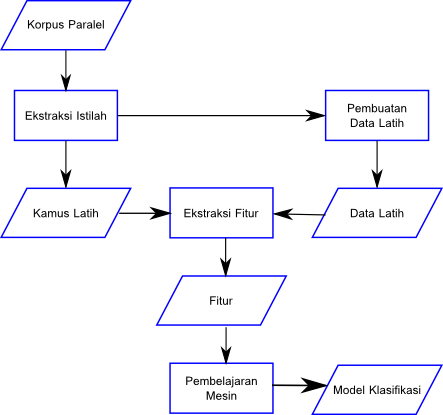
\includegraphics[width=\figurewidth*3/4]{proses_belajar}
	\caption{Desain sistem pembelajaran}
	\label{gbr:solusi_belajar}
\end{figure}

Pelatihan mesin ditujukan untuk menentukan hipotesis yang dapat dipakai untuk membedakan apakah sebuah pasangan istilah merupakan pasangan translasi atau bukan. Sebelum proses ini dilakukan, dibuat terlebih dahulu sebuah kamus latih dan sebuah data latih. Kamus latih dibangkitkan dari sebuah korpus/istilah yang telah \textit{parallel}. Kamus latih digunakan sebagai alat bantu untuk mengekstrak fitur berbasis kamus. Data latih digunakan sebagai acuan penentuan fungsi hipotesis. Keluaran dari proses ini adalah sebuah model klasifikasi. Alur pelatihan mesin beserta dengan praprosesnya diberikan pada Gambar \ref{gbr:solusi_belajar}.

Pada tahap ekstraksi korpus, dilakukan ekstraksi istilah menggunakan GIZA++ dari korpus dwibahasa. Secara ringkas, GIZA++ memasangkan setiap $n$ kata (\textit{$n$-gram}) dari bahasa asal dengan setiap $n$ kata dari bahasa sasaran. Selain itu, dihitung pula frekuensi kemunculannya pada korpus yang dapat dianggap sebagai peluang kemunculan kata tersebut. Alur ekstraksi istilah dari korpus diberikan pada Gambar \ref{gbr:solusi_klasifikasi}.

\begin{figure}[htbp]
	\centering
	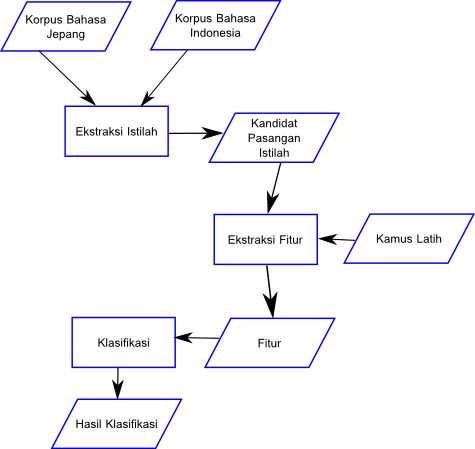
\includegraphics[width=\figurewidth*3/4]{proses_klasifikasi}
	\caption{Desain sistem ekstraksi istilah dari korpus}
	\label{gbr:solusi_klasifikasi}
\end{figure}

\subsubsection{Pembuatan Data Latih}
Data latih diperlukan sebagai bahan pembelajaran. Data latih berupa sebuah daftar pasangan padanan kata/frasa bahasa Indonesia-Jepang yang sudah terdefinisi beserta labelnya (benar/salah). Domain data latih tidak harus sama dengan domain yang dipakai ketika pengujian. Data latih untuk pasangan kata/frasa bahasa Indonesia-Jepang tidak tersedia banyak (atau bahkan tidak ada sama sekali) sehingga perlu penanganan khusus untuk membuatnya. Contoh data latih diberikan pada Tabel \ref{tbl:contoh_entri_data_latih}.

\begin{table}[htbp]
	\centering
	\caption{Contoh entri data latih}
	\label{tbl:contoh_entri_data_latih}
	\begin{tabular}{|l|l|l|}
		\hline
		\textbf{Bahasa Indonesia} & \textbf{Bahasa Jepang} & \textbf{Peluang}\\ \hline
		bahasa & \begin{CJK}{UTF8}{min}言語\end{CJK} & benar\\ \hline
		komputer & \begin{CJK}{UTF8}{min}プログラミング\end{CJK} & salah\\ \hline
		mobil & \begin{CJK}{UTF8}{min}車\end{CJK} & benar\\ \hline
	\end{tabular}
\end{table}

Pembangunan data latih dilakukan dalam 2 proses, yaitu
\begin{inparaenum}[(1)]
\item ekstraksi istilah dari korpus \textit{parallel} dan
\item pelabelan benar/salah secara manual dari hasil yang didapatkan.
\end{inparaenum}
Korpus \textit{parallel} didapatkan dari OPUS sementara ekstraksi istilah dilakukan menggunakan GIZA++. Contoh keluaran GIZA++ diberikan pada Tabel \ref{tbl:contoh_entri_kamus}. Pelabelan benar/salah dilakukan secara manual dengan melihat ke kamus umum bahasa Indonesia-Jepang berdasarkan nilai peluang yang didapatkan dari GIZA++.

\subsubsection{Pembuatan Kamus Latih}
Kamus latih diperlukan untuk mengekstrak fitur berbasis kamus. \textcite{aker} menggunakan GIZA++ untuk membuat kamus latih dengan data diambil dari DGT-TM (\textit{DGT-Translation Memory})\footnote{\url{https://ec.europa.eu/jrc/en/language-technologies/dgt-translation-memory}}. DGT-TM merupakan daftar istilah dalam 22 bahasa berbeda di Eropa yang disusun secara paralel.

Entri dari kamus latih berupa sebuah pasangan kata bahasa Indonesia $I$ dengan kata bahasa Jepang J beserta nilai peluang $p$ dengan $p$ adalah peluang $I$ ditranslasikan menjadi $J$. Contohnya diberikan pada tabel \ref{tbl:contoh_entri_kamus}. Pembuatan kamus latih untuk tugas akhir ini mengikuti cara yang dipakai oleh \textcite{aker}, yaitu menggunakan GIZA++ sedangkan Korpus \textit{parallel} diambil dari OPUS.

\subsubsection{Penyesuaian}
Fitur kognat yang digunakan oleh \textcite{aker} terbagi menjadi 2, yaitu
\begin{inparaenum}[(1)]
\item yang memiliki karakter sama dan
\item yang memiliki karakter berbeda.
\end{inparaenum}
Karena karakter bahasa Indonesia dan bahasa Jepang berbeda, fitur kognat yang memperhitungkan karakter yang sama sudah tidak relevan. Oleh karena itu, hanya dipakai fitur kognat dengan karakter yang berbeda, yaitu yang menggunakan pemetaan karakter.

Penanganan untuk masalah tersebut dilakukan dengan memetakan karakter dari bahasa Jepang (hiragana, katakana, dan Kanji) ke dalam karakter bahasa Indonesia (alfabet). Kakas yang menyediakan pemetaan tersebut banyak tersedia di internet. Salah satunya yang tersedia secara gratis adalah J-Talk\footnote{\url{http://nihongo.j-talk.com/}}.

\subsection{Metode Evaluasi}
Terdapat 2 evaluasi yang dilakukan dalam tugas akhir ini. Yang pertama adalah evaluasi model pembelajaran yang dibuat dengan mengambil data latih sebagai data uji (pengujian tertutup). Yang kedua adalah evaluasi kamus dwibahasa yang didapatkan dari korpus (pengujian terbuka). Kedua evaluasi tersebut dilakukan secara manual dan terbagi ke dalam 2 kasus berikut.

\textbf{Kasus I. Evaluasi Entri Berupa Kata}
\begin{enumerate}
\item Cari kata tersebut di dalam kamus umum bahasa Indonesia-Jepang;
\item Jika kedua kata ditemukan berpasangan, entri dinyatakan benar;
\item Jika tidak ditemukan, entri dinyatakan salah.
\end{enumerate}

\textbf{Kasus II. Evaluasi Entri Berupa Frasa}
\begin{enumerate}
\item Cari frasa tersebut dengan melakukan \textit{query} pada laman web Weblio\footnote{\url{http://ejje.weblio.jp/sentence/}};
\item Jika ditemukan kalimat yang mengandung frasa tersebut dalam bahasa lawannya, entri dinyatakan benar;
\item Jika tidak ditemukan, entri dinyatakan salah.
\end{enumerate}

Selain itu, diadopsi juga sistem evaluasi manual yang dilakukan oleh \textcite{aker} dengan membagi translasi menjadi 2 macam, yaitu translasi penuh dan translasi parsial. Translasi dikatakan penuh jika kedua kata/frasa adalah translasi yang benar. Translasi dikatakan parsial jika terdapat kata yang tidak memiliki translasi dalam bahasa lawannya, namun terdapat juga kata yang memiliki translasi. Translasi parsial hanya mungkin terjadi pada pasangan frasa.

Dalam kasus translasi parsial, pasangan frasa yang terekstrak dianggap sebagai entri yang benar. Oleh karena itu, pada akhir percobaan akan terdapat 2 ukuran, yaitu persentase translasi penuh (hanya menghitung translasi penuh sebagai entri yang benar) dan presentasi translasi parsial (menghitung translasi penuh dan parsial sebagai entri benar).

\end{document}